% don't remove the folling lines, and edit the defintion of \main if needed
\documentclass[../report.tex]{subfiles}
\providecommand{\main}{..}
\IfEq{\jobname}{\currfilebase}{\AtEndDocument{\biblio}}{}
% until here

\begin{document}

\section{Introduction}
\label{sec:Intro}

%\subsection{Executive summary}
%{\bf Abstract:} 
The past decade has witnessed a highly successful programme of flavour physics at the LHC. The unprecedented breadth and precision of the physics results produced by the LHC's dedicated flavour physics experiment, LHCb, has been complemented by crucial measurements at ATLAS and CMS. Together, they have probed the Standard Model at complementary energy scales to the direct LHC searches, and proven that it is possible to carry out a broad programme of precision flavour physics in such a challenging hadronic environment. This document offers a glimpse of the future -- the potential for flavour physics in the High-Luminosity phase of the Large Hadron Collider (HL-LHC) and its possible upgrade to a 27 TeV proton collider, the High-Energy LHC (HE-LHC). 
The landscape of flavour physics is considered and theoretical arguments are presented for measurements with higher precision and of qualitatively new observables.
The prospective experimental sensitivities for the HL-LHC assume 3~ab$^{-1}$ recorded by ATLAS and CMS, and 300~fb$^{-1}$ recorded by a proposed Upgrade II of LHCb.
% In particular, we emphasize the breadth of the flavour physics programme which will be possible at HL-LHC, the wealth of observables which will remain limited by statistics and not theory, and an indirect sensitivity to physics beyond the Standard Model which is highly complementary to direct and high-$p_T$ searches.
%The study covers theoretical as well as specific experimental projections of the relevant experiments, LHCb, ATLAS and CMS. We summarize the main coinclusions, which will be expanded upon in the subsequent sections:
The main points, detailed in the subsequent sections, are:
%\vspace{-\topsep}
\begin{itemize}
\item[$\bullet$]  Flavour physics programme at the LHC comprises of many different probes: the weak decays of  beauty, charm, strange and top quarks, as well as of the $\tau$ lepton and the Higgs;
\item[$\bullet$] Spectroscopy and flavour changing transitions serve as laboratories for better understanding of nonperturbative Quantum Chromodynamics (QCD);
%dynamics of nonperturbative QCD by studying spectroscopy but also the interplay between short- and long-distance physics in hadron decays.
\item[$\bullet$] $\CP$ violation and Flavour Changing Neutral Currents (FCNCs) are sensitive probes of short-distance 
physics, within the Standard Model (SM) and beyond (BSM);
\item[$\bullet$] Flavour physics probes scales $\gg 1$\,TeV, with the  
sensitivity often limited by statistics and not by theory;
\item[$\bullet$] For most FCNC processes a New Physics (NP) contribution at 20\% of the SM is still allowed, so there is plenty of discovery potential;
\item[$\bullet$] Of the several tensions between flavour physics data and the SM, some may soon become decisive;
\item[$\bullet$]  Precision tests of the SM flavour sector will improve by orders of magnitudes including Charged Lepton Flavour Violating transitions (CLFV);
%\item[$\bullet$] There are many challenging theory problems, relevant for improving experimental sensitivity;
\item[$\bullet$]  Flavour physics will teach us about physics at shorter distances, complementary to the high-$p_T$ physics program, whether NP is seen or not, and could point to the next energy scale to explore.
\end{itemize}
%\vspace{-\topsep}


%The past decade has witnessed a highly successful flavour programme at ATLAS, CMS and LHCb. This document offers a glimpse of the future -- the potential for flavour physics in the High-Luminosity phase of the Large Hadron Collider (HL-LHC) and its upgrade to a 27 TeV proton collider, the High-Energy LHC (HE-LHC). 
%The landscape of flavour physics is considered and theoretical arguments are presented for measurements with higher precision and of qualitatively new observables. In particular, we emphasize the breadth of the flavour physics programme which will be possible at HL-LHC, the wealth of observables which will remain limited by statistics and not theory, and an indirect sensitivity to physics beyond the Standard Model which is highly complementary to direct and high-$p_T$ searches.
%The prospective experimental sensitivities for the HL-LHC assume 3~ab$^{-1}$ recorded by ATLAS and CMS, and 300~fb$^{-1}$ recorded by a proposed Upgrade II of LHCb.
%%The study covers theoretical as well as specific experimental projections of the relevant experiments, LHCb, ATLAS and CMS. We summarize the main coinclusions, which will be expanded upon in the subsequent sections:
%%The main points, detailed in the subsequent sections, are:
%%\vspace{-\topsep}
%\begin{itemize}
%\item[$\bullet$]  Flavour physics programme at the LHC comprises of many different probes: the weak decays of  beauty, charm, strange and top quarks, as well as of the $\tau$ lepton and the Higgs;
%\item[$\bullet$] Spectroscopy and flavour changing transitions serve as laboratories for better understanding of nonperturbative Quantum Chromodynamics (QCD);
%%dynamics of nonperturbative QCD by studying spectroscopy but also the interplay between short- and long-distance physics in hadron decays.
%\item[$\bullet$] $\CP$ violation and Flavour Changing Neutral Currents (FCNCs) are sensitive probes of short-distance 
%physics, within the Standard Model (SM) and beyond (BSM);
%\item[$\bullet$] Flavour physics probes scales $\gg 1$\,TeV, with the  
%sensitivity often limited by statistics and not by theory;
%\item[$\bullet$] For most FCNC processes a New Physics (NP) contribution at 20\% of the SM is still allowed, so there is plenty of discovery potential;
%\item[$\bullet$] Of the several tensions between flavour physics data and the SM, some may soon become decisive;
%\item[$\bullet$]  Precision tests of the SM flavour sector will improve by orders of magnitudes including Charged Lepton Flavour Violating transitions (CLFV);
%%\item[$\bullet$] There are many challenging theory problems, relevant for improving experimental sensitivity;
%\item[$\bullet$]  Flavour physics will teach us about physics at shorter distances, complementary to the high-$p_T$ physics program, whether NP is seen or not, and could point to the next energy scale to explore.
%%\end{itemize}
%%\vspace{-\topsep}

\subsection{Theoretical considerations}
%G.\ Isidori, Z.\ Ligeti

As a community we are now in a strikingly different position than we were a decade ago, before the LHC  turned on. 
%it was known that the LHC was essentially guaranteed to obtain a deeper insight into the nature of electroweak symmetry breaking.
%was practically guaranteed. 
%In other words, 
Already before the start of the LHC it was clear from unitarity considerations that the LHC experiments
were basically guaranteed to uncover the origin of the electroweak symmetry breaking, i.e., 
the breaking of the $SU(2)_L \times U(1)_Y$ gauge symmetry to the $U(1)$ of electromagnetism. The discovery of the Higgs boson
by ATLAS and CMS in 2012 was a triumph, vindicating these expectations. Since then we have learned that the properties of the Higgs boson are in increasing
agreement with the SM. Coupled with the lack of direct signals of BSM 
particles so far, this increasingly points to a mass gap between the SM particle spectrum and the BSM one. 
% are some of the first answers the LHC started to provide. 

After completion of the first phase of the LHC program, the field  
entered into a more uncertain, yet possibly more exciting, exploratory era. 
We are still faced by a number of key
open questions, e.g., the need for dark matter and how to generate the baryon asymmetry. We thus do know that BSM physics must exist. However,
% the electroweak hierarchy puzzle, the origin of fermion mass hierarchies, the quantization of $U(1)$ charges), 
we do not know which experiments, at what energy scale, and probing which aspects of our understanding of nature, may provide the first unambiguous evidence for BSM phenomena.
The phenomenological successes of the SM, in conjunction with being a renormalizable quantum field
theory, means that there is no clear guidance where to search for clues on how to extend 
the SM.\footnote{The only clearly established exception 
are neutrino masses, which require non-renormalizable 
operators (or new degrees of freedom) and seem to point toward a very high scale of new physics that is not accessible in practice.
However, 
%if associated with the violation of lepton number,
the existence of a high new scale connected to neutrino mass generation does not prevent other BSM physics to appear at lower scales.}
%%%
This calls for a diversified program of BSM searches, with no stone left unturned. 
A deeper study of the properties of the Higgs boson is one of the pillars of this program, and will be the central focus of the high-luminosity LHC (HL-LHC).  
The same program also offers unique opportunities for tremendous improvements in 
indirect new physics (NP) searches via precision studies of low-energy flavour-changing observables.
Here the expected increase in statistics may be even larger than in the Higgs sector. 
As explained below, this program is complementary to both the high-$p_T$ NP searches, as well as 
to the indirect NP searches performed via the Higgs precision measurements. To show this, we first give 
a brief introduction to flavour physics, starting with the ``flavour problem'', and the general discussion of probing BSM through flavour transitions. 

\smallskip
%{\bf The flavour problem.~~} 
\subsubsection{The flavour problem}
Flavour is the label generically used to differentiate the 12 fermions which, according to the SM, 
are the basic constituents of matter.
These particles can be grouped into 3 families, each containing two quarks and two leptons. The particles within a given family 
have different combinations of strong, weak, and electromagnetic charges. This in turn implies differing behaviors under the SM interactions. 
Across the three families, on the other hand, the particle content is identical except for the masses. That is, in each family we find a set of particles 
with the same SM quantum numbers, but with different masses. 
Ordinary matter consists of particles of the first family: the up and down quarks that form atomic nuclei, as well as the electrons and the corresponding neutrinos.  Why there are three almost identical replicas of quarks and leptons, and the origin of their different mass matrices, 
%  masses and charged current interaction strengths, 
%  GI: I don't like to mention charged-current interaction strengths, 
%  since the strength of the interaction is always the same:
%  the CKM rotation is a pure mass effect. Hope you agree.
%  ZL: How could I not... ;)
is one of the big open questions in fundamental physics, often referred to as the ``SM flavour puzzle''. 

Within the SM, the hierarchy of fermion masses originates from the hierarchy in the strengths of interactions between the fermions and the Higgs field, i.e., from the structure of the Yukawa couplings.  However, this prescription does not provide any explanation  
for the origin of the large hierarchies observed among fermion masses. Putting aside the special case of neutrinos, there are five orders of magnitudes between the mass of an electron and a top quark. Similarly, we do not know what determines the peculiar and rather different mixing structure in the quark and lepton mass matrices, observed through the misalignment of mass and weak-interaction eigenstates in flavour space. 
We do know experimentally, that the Higgs field is responsible for the bulk of the heaviest quark and lepton masses: the top and bottom quarks and the tau leptons. The generation of at least some of the quark masses and mixing angles is thus connected to the Higgs sector. This
suggests a possible connection between the flavour puzzle and the electroweak hierarchy puzzle, 
another big open question pointing toward some form of new physics.

\smallskip
\subsubsection{Model-independent considerations}
The above puzzling aspects make flavour physics, i.e., the precision study of flavour-changing processes in the quark and lepton sector, 
a very interesting window on possible physics beyond the SM.  We do not know if there is an energy scale at which the observed flavour structures assume a simpler form. That is, we do not know if 
 the masses and mixing angles, as observed at low energies, can be predicted in terms of a reduced number of 
more fundamental parameters in a theory valid at some high scale.  On the other hand, precision measurements of flavour-changing transitions may probe such scales, 
even if they are well above the LHC center-of-mass energy.  

This statement can be made quantitative by considering the SM as 
a low-energy effective theory that is valid up to a cut-off scale $\Lambda$, taken to be bigger than the 
electroweak scale $v = (\sqrt{2}\,G_F)^{-1/2} \approx 246$~GeV. 
Under such an assumption of heavy NP, the amplitudes describing a flavour changing transition 
of a fermion $\psi_i$ to a fermion $\psi_j$ 
%(of different flavour) 
can be decomposed in the following general form
\begin{equation}
\mathcal{A}(\psi_i \to \psi_j + X) = \mathcal{A}_{0} \left( \frac{c_{\rm SM}}{v^2} 
+ \frac{c_{\rm NP}}{\Lambda^2} \right) .
\label{eq:fl1}
\end{equation} 
Since in many cases $c_{\rm SM} \ll 1$, NP effects can have a large impact even if $\Lambda \gg v$.
For instance, in the quark sector the reason that often $c_{\rm SM} \ll 1$ is because:
\vspace{-\topsep}
\begin{itemize}
\item[(i)] $c_{\rm SM}$ can be proportional to small 
entries of the Cabibbo-Kobayashi-Maskawa (CKM) matrix and/or to small SM Yukawa couplings; 
\item[(ii)] $c_{\rm SM}$ may include a loop factor $1/(16\pi^2)$, if the corresponding transition is forbidden at tree level, 
as is the case for flavour-changing neutral-current 
(FCNC) transitions or meson-antimeson mixing transitions. 
\end{itemize}
\vspace{-\topsep}
As a result, 
these low-energy processes can probe indirectly, via quantum effects, scales of order $v/\sqrt{c_{\rm SM}}$. These can easily 
exceed those directly reachable via production of on-shell states in current and planned accelerators.
As an explicit example, in the case of $B$\,--\,$\bar B$ mixing, $\sqrt{c_{\rm SM}} \sim |V_{td}|/(4\pi) \sim 10^{-3}$,
hence this observable can probe NP scales up to $10^3$~TeV, in models with $c_{\rm NP} \sim 1$.

The precise values of the NP scale probed at present 
vary over a wide range, depending on the specific observable and the specific NP model
($c_{\rm NP}$ can span a large range, too).
However, the form of Eq.~(\ref{eq:fl1}) does allow us to predict how the bounds will 
improve with increasing data sets. For the observables that are SM dominated, are already observed, 
and whose uncertainties are dominated by statistics,
the corresponding bound on $\Lambda$ scales as $N^{1/4}$, 
where $N$ is the relative increase in the number of events.
The same scaling occurs for forbidden or highly suppressed SM processes, i.e., in the limit $c_{\rm SM} \ll c_{\rm NP}$,
if the search is not background dominated. 
Thus, with two orders of magnitude increase in statistics one can probe scales roughly 3 times higher
than at present. This is well above the increase in NP scale probed in on-shell heavy particle searches at high-$p_T$ that can be achieved at fixed collider energy by a similar increase in statistics.

While theoretical uncertainties are often important, there are enough measurements which are known 
not to be limited by theoretical uncertainties. Improved experimental results will therefore directly translate to better NP sensitivity.  
There are also several cases of observables sensitive to NP where the theoretical uncertainties  
are mainly of parametric nature (e.g., our ability to precisely compute $c_{\rm SM}$ is dominated by the knowledge of CKM elements, 
quark masses, etc.). For such cases we can expect significant increase in precision with higher 
statistics, thanks to the improvement in the reduction of parametric uncertainties. This also highlights the importance of a broad 
flavour physics program, where the focus is not only on rare or $\CP$ violating processes, ``most likely'' affected by NP,
but also on core SM measurements, which help to reduce the theoretical uncertainties. 

\smallskip
\subsubsection{Nonperturbative QCD and its role in flavour physics} Of special interest are the theoretical uncertainties due to our incomplete understanding of QCD dynamics at low energies. In order to extract information on short-distance physics from weak decays of hadrons, knowledge of nonperturbative matrix elements, encoded in decay constants and form factors, is needed. 
%The last decade has also witnessed important theoretical progress in the calculation of these hadronic parameters, with 
Refinements in the effective-field-theory (EFTs) approaches exploiting heavy-quark and/or low-energy perturbative expansions and, specially, major progress in the maturity of lattice QCD calculations seen in the last decade, make the BSM flavour physics programme possible. Some of the hadronic inputs have already reach the per-mille level, e.g., the theoretical precision in the calculation of nonperturbative quantities crucial for the extraction of the CKM matrix element $|V_{us}|$, the theory prediction for the rare FCNCs decay $B\to\mu\mu$. 

On the other hand, there are many other transitions 
%e.g., the  non-leptonic decays,that are still not accessible to lattice calculations, and 
that would benefit from further theoretical break-throughs. 
%. The understanding of these quantities also benefits from the breadth of the experimental flavor physics program in the HL-LHC as many can be interconnected by using theoretical methods that exploits symmetries (such as EFTs) or dispersive techniques. 
In the past, large increases in available data always triggered new theory developments, and better understanding of the domain of applicability and accuracy of existing theoretical tools.  It can be anticipated that these fruitful cross-fertilizations will continue to occur in the HL-LHC era between flavour physics experiments and theory.  While there is a substantial suite of measurements whose interpretations will not be limited by hadronic uncertainties, the experimental program can still benefit a lot from theoretical improvements.  For many observables, anticipated lattice QCD improvements are important.  The anticipated improvements in experimental precision also pose interesting challenges for lattice QCD, to robustly address isospin violating and electromagnetic effects in flavour observables.  For many nonleptonic decays, relevant for $CP$ violation, lattice QCD is unlikely to make a big impact. Nevertheless, developing new methods based on effective theories and testing existing approaches can be expected to improve the theoretical understanding of many observables, further enhancing the sensitivity of the experimental program to possible BSM phenomena.

Understanding the nonperturbative structure of QCD of course has tremendous scientific merit per se, decoupled from the searches for NP. A very active area of research that will benefit from flavour programme at HL- and HE-LHC
%A part of the flavour-physics experimental program that is shedding light into the dynamics of nonperturbative QCD 
is hadron spectroscopy. A plethora of exotic states, many of which were unexpected or show intriguing features, have been discovered at the $B$-factories and the LHC. The increase of data samples at the HL-LHC will allow to discover many more of these states and chart their quantum numbers and properties. Accommodating them into the our theoretical understanding of the nonperturbative regime of QCD will be a major challenge for the next decade. 
%In turn, the knowledge thus gained, will be certainly useful in the interpretation of certain weak hadron decays in terms of the short-distance physics (e.g. in charm-loop contributions to $B\to K^{(*)}\ell\ell$ decays). 



\smallskip
\subsubsection{Current anomalies and historical comments}
Due to the generic sensitivity to high scales, flavour physics has historically played a major role in developing and understanding 
the Standard Model. Flavour physics measurements signaled the presence of ``new'' particles 
well before these were directly observed (this was the case for charm and top quarks from $K$-meson and $B$-meson mixing, respectively). 
With the completion of the SM, and the increasingly precise tests its predictions passed, one may draw a naive conclusion that the discovery potential of precision experiments declined in the last decades. 
However, quite the opposite is true. First of all, a qualitative change in our understanding has been achieved during that time. Before the asymmetric $B$ factory experiments, BaBar and Belle, it was not known whether the SM accounted for the dominant or maybe just a small part of $CP$ violation observed in kaon mixing and decay.  We now know that the bulk of it is due to the SM Kobayashi-Maskawa mechanism. On the other hand, 
even after decades of progress, for most FCNC amplitudes the NP is still allowed to contribute at $\sim$\,20\% of the SM contribution.

The great improvements in precision for several flavour-changing process achieved in the last 20 years, both at experimental and theoretical level, represents a very important advancement of the field. 
We learned that either NP is much heavier than the electroweak scale,
or, if it is not far above the electroweak scale as required by most solutions of the hierarchy puzzle, it must have a highly 
nontrivial flavour structure, able to mimic the strong suppression of flavour-changing neutral-current transitions in the SM.
The latter statement has often been oversimplified, assuming that there is little hope to observe significant deviations from the SM in  
flavour physics. The anomalies recently observed in semileptonic $B$ decays clearly demonstrated a genuine discovery potential, whether their significance increase or decrease with improved measurements.

Recent measurements, both in charged- and in neutral-current 
semileptonic $B$ decays, hint at a violation of one of the 
key predictions of the SM -- the universality of interactions for leptons of different generations
(in the limit where their masses can be neglected).  These anomalies represent the strongest tensions
with the SM predictions currently observed in laboratory experiments. The statistical significance of the anomalies is not high enough to 
claim a discovery, but the situation is very interesting. 
More precise measurements of some of these observables, in particular the lepton flavour universality violating ratios
$R_{K^{(*)}} = \Gamma(B\to K^{(*)} \mu^+\mu^-) / \Gamma(B\to K^{(*)} e^+e^-)$ and 
$R(D^{(*)}) = \Gamma(B\to D^{(*)} \tau\bar\nu) / \Gamma(B\to D^{(*)} l\bar\nu)$, where $l=e,\, \mu$,
could establish the presence of new physics even 
with modest improvements in statistics.  At the current central values for these anomalies, 
analyzing all of the Run~1 and Run~2 data could already establish a discrepancy with the SM expectation 
in a single observable with $5\,\sigma$ significance.

Whether or not these anomalies will gain significance to become unambiguous signals of physics beyond the SM, 
they have clearly exemplified the discovery potential of flavour-physics observables, 
and enlarged our horizon regarding possible BSM scenarios. Before the appearance of these anomalies, 
lepton flavour universality (LFU) was an implicit assumption adopted by the vast majority of proposed BSM scenarios.
It is now better appreciated that LFU is an accidental property of the SM. It is well tested in transitions involving only 
the first two generations of quarks and leptons, while it is rather poorly tested in processes involving the third generation 
(and may indeed be violated at a detectable level in $B$ decays). A deeper scrutiny of this SM property has highlighted 
the interest in a large variety of observables, with small theoretical uncertainties, which would strongly benefit from more statistics. 
Similarly, it was often taken for granted that NP 
effects in tree-level dominated processes, such as those affecting $R(D^{(*)})$, are negligible, while it is now clear that 
there exist NP scenarios where this assumption might not hold. This observation has important 
 phenomenological consequences, and signals the limitation of a significant fraction of current NP analyses.
Last but not least, theoretical models addressing the anomalies have highlighted the  interest of BSM constructions
containing heavy leptoquark fields -- a class of NP models that was not popular until a few years ago. 

The current central values of $R_{K^{(*)}}$ and, especially, $R(D^{(*)})$ imply that NP needs to be at a fairly low scale: below few tens of TeV in the former,  
and a few TeV in the latter case.  This can be easily understood, given that the NP effects need to give ${\mathcal O}(10\%-20\%)$ corrections to the amplitudes which are one-loop and tree level in the SM, respectively. Models addressing the anomalies are therefore a perfect laboratory to explore the interplay between 
indirect NP searches from flavour observables and direct searches at high-$p_T$. Interestingly enough, even in the low-scale models 
addressing $R(D^{(*)})$, with or without $R_{K^{(*)}}$, there exist ample regions of parameter space 
able to explain the anomalies, that are at the same time consistent with the null results of NP searches performed so far at the high-$p_T$.

\smallskip
\subsubsection{Connections to lepton flavour violation}
The charged lepton flavour violating (CLFV) processes, such as $\tau \to 3 \mu$, 
are essential parts of the flavour-physics program.  
CLFV amplitudes can also be decomposed as in Eq.~(\ref{eq:fl1}), with the advantage that in this case 
$c_{\rm SM}$ vanish.  If the SM is extended to describe neutrino masses, non-zero predictions arise, 
but are suppressed by $m_\nu^2$. The predicted CLFV rates are thus many orders of magnitudes below the 
detection reach of any present or planned facility. As a consequence the searches for CLFV are very clean 
and powerful ways to search for physics beyond the SM.

Any attempt to solve the flavour puzzle with new dynamics not far from the TeV scale, such that  the observed hierarchies in the Yukawa couplings are accounted for by the new dynamics, 
%(i.e., where new dynamics account for )
unavoidably leads to CLFV rates not far from the present bounds. The recent LFU anomalies 
have strengthened the case further: virtually all models explaining these anomalies predict 
CLFV at at detectable level, in many cases just below the current bounds. 
Of noteworthy interest, triggered by the recent anomalies, are processes 
that violate both quark and lepton flavour, such as $B \to K \tau \mu$.  
There is a large variety of observables of this type that, together with purely leptonic observables, 
form a large and very promising sub-field of new physics probes. Such searches can be organized 
in a large matrix, with the row and column indices determined by lepton and quark flavours, which is largely unexplored at present. For any NP model that may populate entries in this matrix, there is a large  
%and exhibits the 
complementarity between the HL-LHC
experiments, Belle~II, and dedicated experiments at muon beams searching for 
$\mu\to e$ conversion, $\mu\to e\gamma$, and $\mu\to 3 e$.

\smallskip
\subsubsection{Connections with the hierarchy problem and complementarity with high-$p_T$ searches} 
BSM models proposed to address the electroweak hierarchy problem, such as supersymmetric models or composite models, predict new particles around the TeV scale. For all these models, flavour physics imposes very stringent bounds, requiring a flavour structure not far from that in the SM. This was the main rationale underlying 
the hypothesis of Minimal flavour Violation (MFV). The MFV hypothesis is an ansatz for the flavour structure of NP that assumes that the SM Yukawa couplings are the only sources of flavour non-degeneracy even beyond the SM.
This requirement is nowadays partially relaxed by the absence of direct signals of NP in high-$p_T$ experiments, allowing non-trivial modifications from the strict MFV.
This example illustrates nicely the importance of flavour physics in reconstructing the structure of any NP model addressing the electroweak hierarchy problem, but also its complementarity with the high-$p_T$ experiments, where improved direct bounds relax the flavour structure requirements.

If there are new particles which couple to the SM quarks or leptons,  then, in general, there are corresponding new flavour parameters. Measuring them would be very important in order to understand the structure of new physics.  This has been studied in great detail in the context of SUSY (alignment mechanism
of the soft-breaking terms), and in composite models 
(partial-composite mechanism).
In the specific case of low energy supersymmetry, the squark and slepton couplings may yield measurable effects in FCNC processes and $CP$ violating observables, and may give rise to detectable CLFV transitions.  Observable $CP$ violation is also possible in neutral currents and in electric dipole moments, for which the SM predictions are below the near future experimental sensitivities. The supersymmetric flavour problems, namely the 
observation that TeV-scale SUSY models with generic parameters are excluded by FCNC and $CP$ violation measurements, can be alleviated in several scenarios: (i) universal squark masses (e.g., gauge mediation); (ii) quark--squark alignment, (e.g., horizontal symmetry); (iii) very heavy squarks (e.g., split SUSY). All viable models incorporate some of these ingredients. Conversely, if SUSY is discovered, mapping out its flavour structure, with the help of future more precise flavour tests,
may help answer questions about even higher scales, the mechanism of SUSY breaking, how it is communicated to the MSSM, etc.



\smallskip
\subsubsection{Unexpected discoveries}
It goes without saying that it is impossible to predict truly unexpected future discoveries.  However, it cannot be emphasized enough that the large increase in data sets has the potential to revolutionize the field by unexpected discoveries, and trigger entirely new areas of experimentation.  It should be obvious that exact and approximate conservation laws should be tested as precisely as possible, especially when the experimental sensitivity can substantially increase.  Recall that the discovery of $CP$ violation itself was unexpected, in an experiment whose primary goal was checking an anomalous kaon regeneration result.  New particles with surprising properties were in fact discovered at each of BaBar, Belle, and LHCb; respectively, the discoveries of the $D_{sJ}(2317)$ meson with a mass much below expectations, the discovery of the unexpectedly narrow charmonium-like state $X(3870)$ and the $Z(4430)$, and the discovery of pentaquarks.  Thus, beside the``classical'' searches for flavour-violating processes mentioned so far, both in quark and lepton sectors, other searches such as the searches for dark sectors in many channels, or not yet conceived BSM searches, will all form important parts of the flavour physics program in the HL-LHC era.

%\smallskip
%{\bf Theory improvements.~~} 
%In the past, large increases in available data always triggered new theory developments, and better understanding of the domain of applicability and accuracy of existing theoretical tools.  It can be anticipated that these fruitful cross-fertilizations will continue to occur in the HL-LHC era between flavour physics experiments and theory.  While there is a substantial suite of measurements whose interpretations will not be limited by hadronic uncertainties, the experimental program can still benefit a lot from theoretical improvements.  For many observables, anticipated lattice QCD improvements are important.  The anticipated improvements in experimental precision also pose interesting challenges for lattice QCD, to robustly address isospin violating and electromagnetic effects in flavour observables.  For many nonleptonic decays, relevant for $CP$ violation, lattice QCD is unlikely to make a big impact. Nevertheless, developing new methods based on effective theories and testing existing approaches can be expected to improve the theoretical understanding of many observables, further enhancing the sensitivity of the experimental program to possible BSM phenomena.

\smallskip
\subsection{Experimental considerations and the breadth of flavour physics} 
Between now and the end of the HL-LHC, the useful data sets will increase by a factor of order 30--50, however, due to improvements in detector capabilities and changing running conditions, robust estimates of sensitivity improvements are complicated tasks left for detailed studies in the next sections.  At LHCb, in most analyses, one may expect faster improvements in the results than simply scaling with collected total luminosity, due to improvements in detector capabilities in the upcoming upgrades.
At ATLAS and CMS the large number of interactions per bunch crossing during the HL-LHC will be a challenge. Nevertheless, it is important pursue as broad a program as possible, since several key channels are expected to remain competitive with LHCb.
In many cases Belle~II will provide competition and cross-checks of LHCb results.  However, especially in the very low rate modes, such as $B_d\to \mu^+\mu^-$, it is ATLAS and CMS and not Belle~II which are expected to best compete with LHCb.  If there are anomalies in $B_s$, and especially in $\Lambda_b$ decays, they can only be cross-checked at the LHC experiments.
 
As mentioned above, our ignorance about BSM physics requires a diversified program that,  
even within the flavour-physics domain, calls for a large set of complementary measurements. 
These cannot all be 
performed at a single facility. There is full complementarity, and many potential synergies 
in case some BSM signal emerges, among different $b$-hadron decays ($B_{u,d}$, 
$B_s$, $\Lambda_b$, etc.), $CP$ violating and rare processes involving  
charm and kaons, as well as possible FCNC top-quark decays. 
\smallskip




%%%%%%%%%%%%%%%%%%%%%%%%%%
%%%%%%%%%%%%%%%%%%%%%%%%%%


\subsubsection{Key experimental capabilities at ATLAS and CMS}
%{\bf EXP Author(s): S.\ Malvezzi, A.\ Cerri } 
%S.\ Malvezzi, A.\ Cerri

The high-luminosity LHC upgrade (HL-LHC) will allow to deliver to the CMS and ATLAS experiments proton-proton collisions at a center-of-mass 
energy of 14 TeV for a total integrated luminosity of about 3000\,fb$^{-1}$. 
 This goal will be achieved through a high instantaneous luminosity which implies up to 200 proton-proton interactions in each collision. In this regime, the experimental sensitivity to new physics is enhanced and complemented by flavour physics measurements, with sensitivities in specific modes 
(e.g., $B_{s,d} \to \mu\mu$ and $B_s \to J/\psi \phi$) comparable to those of dedicated experiments.
The ability of general purpose detectors to make precision heavy flavour measurements has been clearly demonstrated
%definitely proven 
by the results from Run~1 and Run~2 data.
HL-LHC can be a unique test bench for $B$ physics studies in ATLAS and CMS: $\sim$ 10$^{15}$ $b\bar{b}$ pairs will be produced for the integrated luminosity goal.

It is not however trivial for ATLAS and CMS to fully exploit this potential: $B$ physics is expected to be 
among the areas that may suffer most heavily from the HL-LHC conditions. This is a consequence of the relatively 
low momenta of typical heavy flavour signatures, and the high pile-up which might affect the precision of the measurements.
On the other hand, some projected Phase-II upgrades of ATLAS and CMS promise good detection potential, good pile-up mitigation and even -- in some cases -- an improved performance. Examples are the new inner trackers, improvements of the muon systems, topological trigger capabilities, and the possibility to use tracking in the early stages of the trigger chain.
 
The expected high integrated luminosity will allow ATLAS and CMS to study some rare processes at a precision never attained before. The excellent tracking and muon identification performances are highlighted by a number of  benchmark channels, $B_{s,d} \to \mu\mu$, $B^0 \to K^{*0} \mu\mu$, $B_s \to J/\psi \phi$, and $\tau \to 3\mu$, that are used for projections. 
Precision measurements at the level of 5\% to 10\% for the $B^0_s \to \mu^+\mu^-$  branching fraction, %of about 7\%, 
are expected, along with the observation of the 
$B^0 \to \mu^+ \mu^-$ with more than 5$\sigma$, and a measurement of the $B^0_s \to \mu^+\mu^-$ effective lifetime with an uncertainty of 0.05 ps.
The sensitivity to the CP-violating phase $\phi_s$ in the $B^0_s \to J/\psi \phi(1020)$ mode is estimated to be at the level of $\sim$ 5 mrad, 
i.e., a factor of $\sim$ 20 better than the corresponding Run~1 analyses values (a factor of $\sim 5 $ with respect to the combined $b \to \bar c c s$ measurements). 
The uncertainty on the angular variable $P_5'$ in the $B^0 \to K^{*0} \mu^+ \mu^-$  as a function 
of the dimuon squared invariant mass ($q^2$ ) is expected to improve up to a factor of 15 with respect to the published Run~1 measurements; 
with the HL-LHC high statistics the $B^0 \to K^{*0} \mu^+ \mu^-$ analysis can be performed in narrow bins of $q^2$ to reach a more precise determination of the angular observables.
Finally, the $\tau \to 3 \mu$ decay is expected to be probed down to $\mathcal{O} (10^{-9})$.

%\td{we will see in a month from now what we have in hands}
The lack of particle-ID detectors is bound to limit the investigation of fully hadronic final states at ATLAS and CMS. Nevertheless, some capability is retained through the early use of tracking in the trigger selection.  The $B_s \to \phi \phi \to 4K$ decay is an example of a hadronic final state that would benefit from the tracking performance at trigger level and the $\phi$ resonance signature.
 
The heavy flavour program at ATLAS and CMS requires dedicated low $p_T$ triggers, in contention for bandwidth with high $p_T$ measurements and searches. The physics scenario at the time of HL-LHC will motivate the optimal trigger bandwidth allocation for low $p_T$ studies.%, driven by physics goals.% and optimal trigger performance.
The high $p_T$ searches in ATLAS and CMS will also allow for a program of measurements which are complementary to the low $p_T$ flavour investigations and will help to build a coherent theoretical picture. 
%\td{wait to see how it will be discussed in the dedicated chapters}
 
%\td{Include abstract-like summary of results discussed, %once results available are fully defined.}

%\clearpage
\subsubsection{Key experimental capabilities at LHCb}
The Upgrade II of LHCb will enable a very wide range of flavour observables to be determined with unprecedented precision, which will give the experiment sensitivity to New Physics scales several orders of magnitude above those accessible to direct searches. 
The expected uncertainties for a few key measurements  with 300\invfb are presented in Table~\ref{tab:physummary}. The future LHCb estimates are all based on extrapolations from current measurements, and take no account of detector improvements apart from an approximate factor two increase in efficiency for hadronic modes, coming from the full software trigger that will be deployed from Run 3 onward. Three principal arguments motivate the Upgrade II of LHCb, and the full exploitation of the HL-LHC for flavour physics.
\begin{enumerate}
\item
There is a host of measurements of {\it theoretically clean} observables, such as the \CP-violating phase $\gamma$, the lepton-universality ratios $R_K$, $R_{K^\ast}$ {\it etc.}, or the ratio of branching fractions $R\equiv {\cal{B}} (\Bd \rightarrow \mu^+ \mu^-)$/${\cal{B}} (\Bs \rightarrow \mu^+ \mu^-)$, where knowledge will still be statistically limited after Run~4.  The same conclusion applies for other observables such as $\phi_s$ and $\sin 2 \beta$, where strategies exist to monitor and control possible Penguin pollution. The HL-LHC and the capabilities of LHCb Upgrade II offer a unique opportunity to take another stride forward in precision for these quantities.  Advances in lattice-QCD calculations will also motivate better measurements of other critical observables, {\it e.g.} $|\Vub|/|\Vcb|$.  

The anticipated impact of the improved knowledge of Unitarity Triangle parameters can be seen in Fig.~\ref{fig:UTprojection}, which shows the evolving constraints in the $\bar{\rho}-\bar{\eta}$ plane from LHCb inputs and lattice-QCD calculations, alone.   The increased sensitivity will allow for extremely precise tests of the CKM paradigm. In particular, it will permit the tree-level observables, which provide Standard-Model benchmarks, to  be assessed against  those with loop contributions, which are more susceptible to New Physics.  In practice, this already very powerful ensemble of constraints will be augmented by complementary measurements from Belle II, particularly in the case of $|\Vub|/|\Vcb|$.

The increasing precision of observables from measurements of statistically-limited FCNC processes will provide significant improvements in sensitivity to the scale of New Physics.  As an example, Table~\ref{tab:wilson_sum} shows the expected improvement with integrated luminosity in the knowledge of the Wilson coefficients $C_9$ (vector current) and $C^\prime_{10}$ (right-handed axial-vector current), and the corresponding 90\% exclusion limits to the New Physics scale $\Lambda_{\rm NP}$ under various scenarios. The reach for generic New Physics at tree-level in Upgrade~II is found to exceed 100~TeV. 

\item
It will be essential to {\it widen the set of observables under study} beyond those accessible at the current LHCb experiment or its first upgrade, {\it e.g.} by including additional important measurements involving  $b \to s/d \ellell$ and $b \to c \ell^-\bar{\nu_l}$ decays.  Improving our knowledge of the flavour sector both through better measurements and through new observables will be essential in searching for, and then characterising, New Physics in the HL-LHC era.

\item
Due to its ability to reconstruct and analyze all collisions in real-time, and the statistical power of the HL-LHC dataset, LHCb \upgradetwo will be able to collect a unique dataset for hadronic spectroscopy. This will enable not only the precise understanding of excited mesons and conventional baryons, but also a detailed and broad understanding of tetraquarks, pentaquarks, baryons containing multiple heavy quarks, and other yet-to-be-discovered exotic states of quark matter. While not directly sensitive to BSM effects, these measurements will play an important role in sharpening our understanding of QCD at the energy scales relevant for flavour physics, and hence make an important contribution to the accurate interpretation of any observed BSM anomalies. 
\end{enumerate}
%The improvement in physics reach between Upgrade I and Upgrade II will be greater than the simple factor of six in integrated luminosity would indicate (or factor 13, when integrating from Run 4 onward).  
The intention to operate a flavour-physics experiment at luminosities of $10^{34}\,{\rm cm^{-2}s^{-1}}$ is already an ambitious one, but the planned improvements to the detector's capabilities will extend the physics gains still further.  These gains are not included in Table~\ref{tab:physummary} as full simulations have not yet been performed,  but a summary of the expected benefits can be found in~\cite{Bediaga:2018lhg}. It is intended to take first steps towards some of these detector enhancements already in LS3, before the start of the HL-LHC , thereby improving the performance of the first LHCb upgrade, and laying the foundations for Upgrade II. Finally, it must be emphasised that the raw gain in sample sizes during the HL-LHC era will have great consequences for the physics reach, irrespective of any detector improvements.   The energy scale probed by virtual loops in flavour observables will rise by a factor of up to 1.9 with respect to the pre-HL-LHC era, with a corresponding gain in discovery potential that is similar to what will apply for direct searches if the beam energy is doubled, as proposed for the HE-LHC.

\begin{table}[ptb!]
\caption{\small Summary of prospects for future measurements of selected flavour observables for LHCb.  The projected LHCb sensitivities take no account of potential detector improvements, apart from in the trigger.\vspace*{0.1cm}}\label{tab:physummary}
\centering
\begin{tabular}{lrrr} \hline\hline
Observable  &   Current LHCb  &  LHCb 2025  &  Upgrade II  \\ \hline
%
\underline{\bf EW Penguins}  &  & & \\
$R_K$ $(1<q^2<6\,{{\rm GeV}^2c^4})$            & 0.1\cite{LHCb-PAPER-2014-024}  &  0.025   &   0.007  \\
$R_{K^\ast}$ $(1<q^2<6\,{{\rm GeV}^2c^4})$  & 0.1\cite{LHCb-PAPER-2017-013}  &  0.031  &   0.008 \\
$R_\phi$,  $R_{pK}$, $R_{\pi}$         & -- & 0.08, 0.06, 0.18 & 0.02, 0.02, 0.05 \\
%
\rule{0pt}{3ex}\underline{\bf CKM tests}  &   & &\\
%
$\gamma$, with $\Bs \to \Ds\Km$ & $(^{+17}_{-22})^\circ$~\cite{LHCb-PAPER-2017-047} & 4$^\circ$ & 1$^\circ$ \\
$\gamma$, all modes & $(^{+5.0}_{-5.8})^\circ$~\cite{LHCb-CONF-2018-002} & 1.5$^\circ$ & $0.35^\circ$ \\
$\sin 2 \beta$, with $\Bd \to J/\psi\KS$ & $0.04$\cite{LHCb-PAPER-2017-029} & $0.011$ & $0.003$ \\
$\phi_s$, with $\Bs \to J/\psi \phi$ & 49 mrad\cite{LHCb-PAPER-2014-059}  & 14 mrad  & 4 mrad \\
$\phi_s$, with $\Bs \to \Dsp\Dsm$   & 170 mrad\cite{LHCb-PAPER-2014-051}  & 35 mrad  & 9 mrad \\
%$\phi_s^{s{\bar{s}s}}$, with $\Bs \to \phi\phi$  & 150 mrad\cite{LHCb-PAPER-2014-026} & 60 mrad & --  & 17 mrad  & Under study~\cite{CMS-PAS-FTR-16-006}\\
$\phi_s^{s{\bar{s}s}}$, with $\Bs \to \phi\phi$  & 154 mrad\cite{LHCb-PAPER-2014-026} & 39 mrad & 11 mrad \\
%$a^d_{sl}$ & $36 \times 10^{-4}$\cite{LHCb-PAPER-2014-053}  &    $8 \times 10^{-4}$    &  $1 (?) \times 10^{-4}$ & $2 \times 10^{-4}$ & \\
$a^s_{\rm sl}$ & $33 \times 10^{-4}$\cite{LHCb-PAPER-2016-013}  &  $10 \times 10^{-4}$  & $3 \times 10^{-4}$\\
$|\Vub|/|\Vcb|$  & 6\%\cite{LHCb-PAPER-2015-013}  & 3\%   & 1\% \\
%
%
\rule{0pt}{3ex}\underline{\bf ${\bm{B^0_s, B^0} {\to} \bm{\mu^+}\bm{\mu^-}}$}  &  & \\
${\cal{B}} (\Bd \rightarrow \mu^+ \mu^-)$/${\cal{B}} (\Bs \rightarrow \mu^+ \mu^-)$ & 90\%\cite{LHCb-PAPER-2017-001}  & 34\%  & 10\% \\
$\tau_{\Bs \to \mu^+\mu^-}$ &22\%\cite{LHCb-PAPER-2017-001} & 8\%  & 2\% \\
$S_{\mu\mu}$ & -- &  -- & 0.2\\
%                      
\rule{0pt}{3ex}\underline{\bf\boldmath {${b \to c \ell^-\bar{\nu_l}}$} LUV studies}  &    & \\
$R(D^\ast)$ & 0.026\cite{LHCb-PAPER-2015-025,LHCb-PAPER-2017-027}  & 0.0072 & 0.002\\
$R(J/\psi)$ & 0.24\cite{LHCb-PAPER-2017-035} & 0.071 & 0.02 \\
%
\rule{0pt}{3ex}\underline{\bf Charm}  &   &  &\\
$\Delta A_{\CP}(KK-\pi\pi)$ &  $8.5 \times 10^{-4}$\cite{LHCb-PAPER-2015-055}  & $1.7\times 10^{-4}$ &  $3.0 \times 10^{-5}$ \\
$A_\Gamma$ ($\approx x \sin\phi$) & $2.8 \times 10^{-4}$\cite{LHCb-PAPER-2016-063} & $4.3 \times 10^{-5}$ &  $1.0 \times 10^{-5}$ \\
${x \sin \phi}$ from $\Dz \to K^+\pi^-$ & $13\times 10^{-4}$\cite{LHCb-PAPER-2017-046} & $3.2 \times 10^{-4}$ & $8.0 \times 10^{-5}$ \\
${x \sin \phi}$ from multibody decays & -- & ($K3\pi$) $4.0\times 10^{-5}$ & ($K3\pi$) $8.0 \times 10^{-6}$ \\
%\rule{0pt}{3ex}\underline{\bf Photon polarisation}  &   &  & & & -- \\
\hline\hline
\end{tabular}
\end{table}
\clearpage


\begin{figure}[H]
\begin{center}
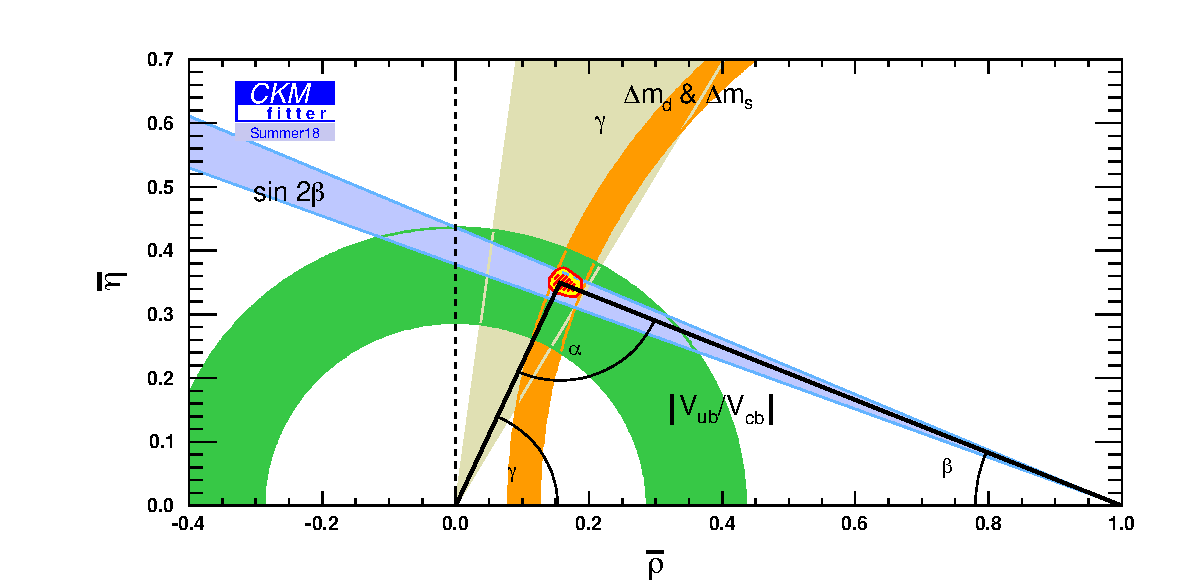
\includegraphics[width=0.75\textwidth]{section1/figs/rhoeta_small_LHCb_Summer18.pdf}

\begin{minipage}{0.75\textwidth}
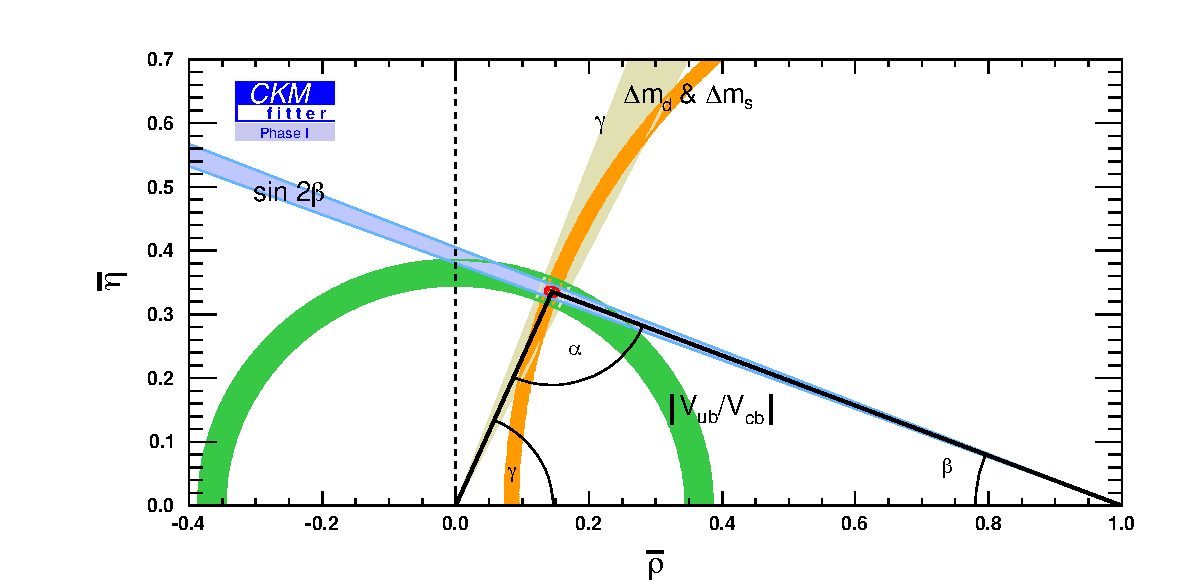
\includegraphics[width=\textwidth]{section1/figs/rhoeta_small_LHCb_Stage1.pdf}\vspace{-5.36cm}
\mbox{\hspace{7.9cm}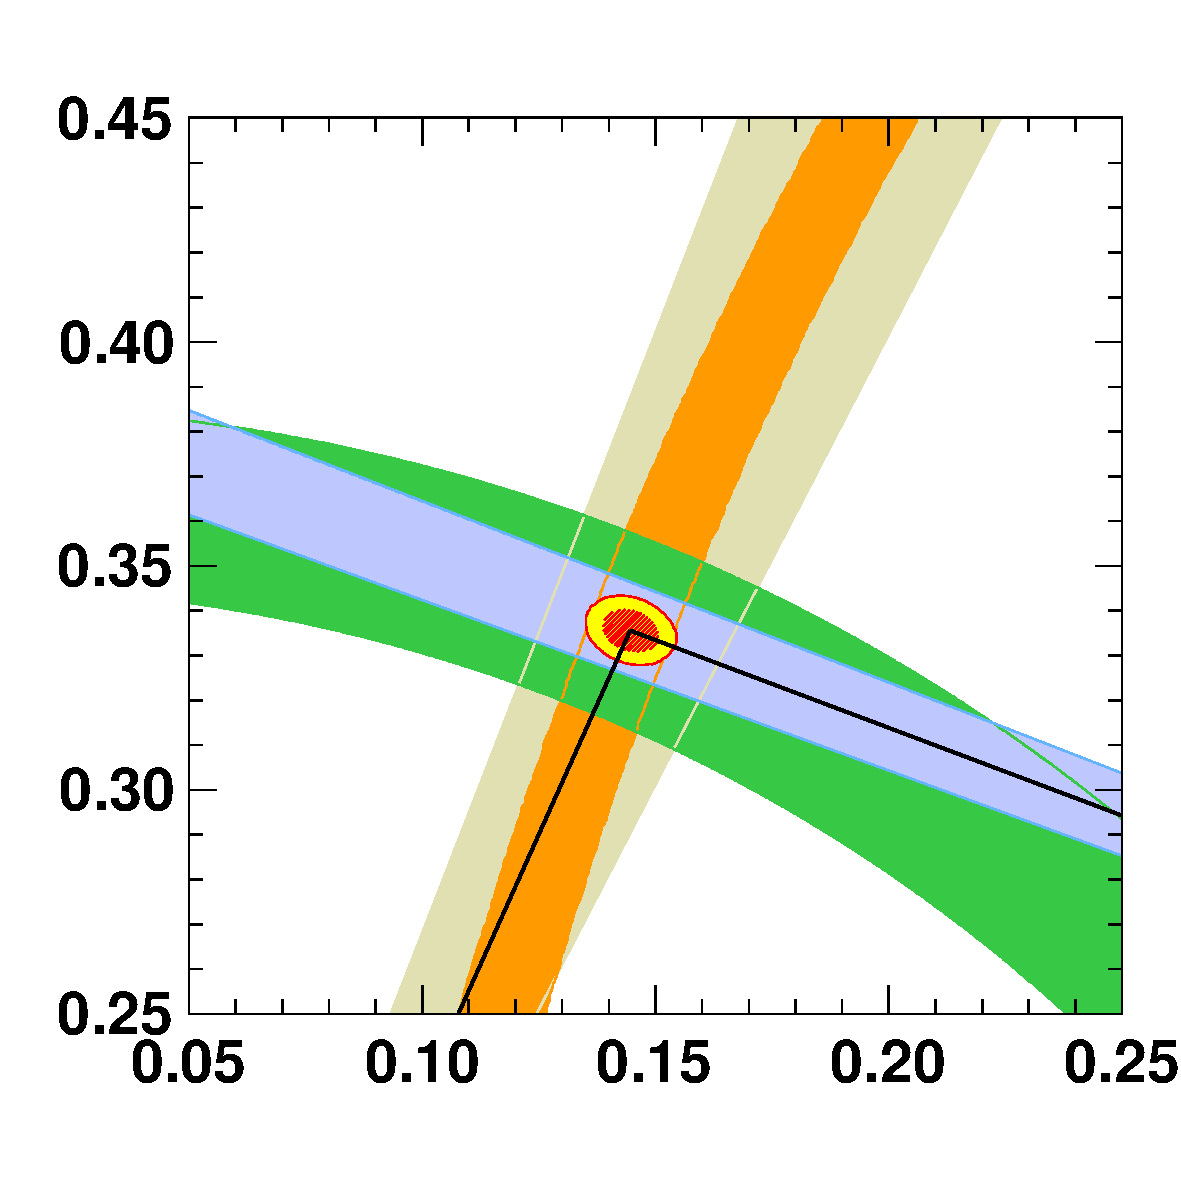
\includegraphics[width=0.26\textwidth]{section1/figs/rhoeta_small_zoom_LHCb_Stage1.pdf}}
\vspace{2.25cm}
\end{minipage}

\begin{minipage}{0.75\textwidth}
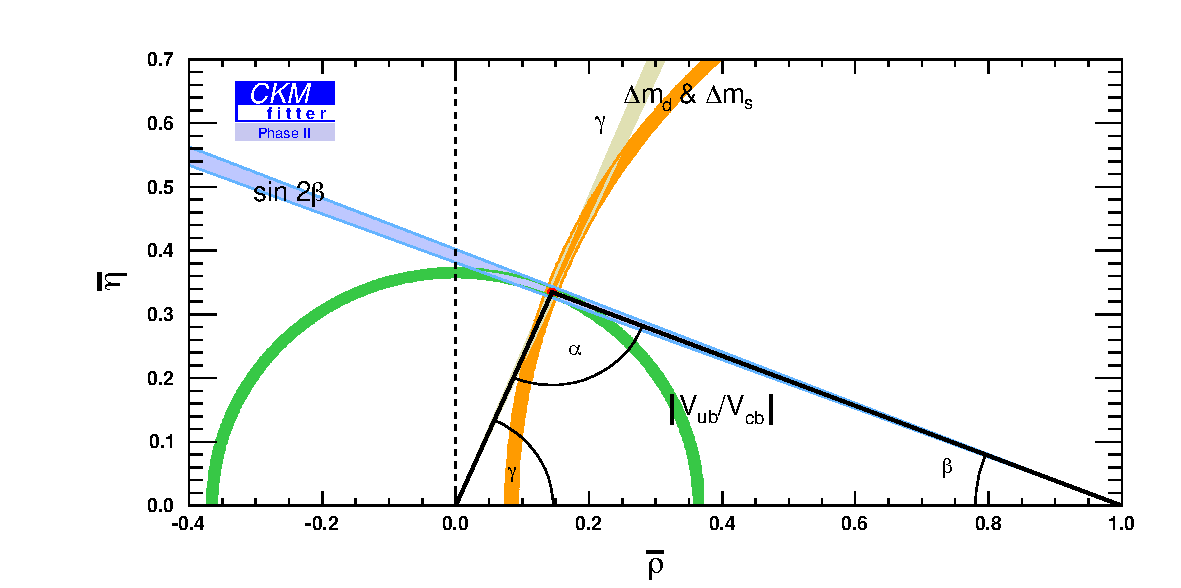
\includegraphics[width=\textwidth]{section1/figs/rhoeta_small_LHCb_Stage2.pdf}\vspace{-5.36cm}
\mbox{\hspace{7.9cm}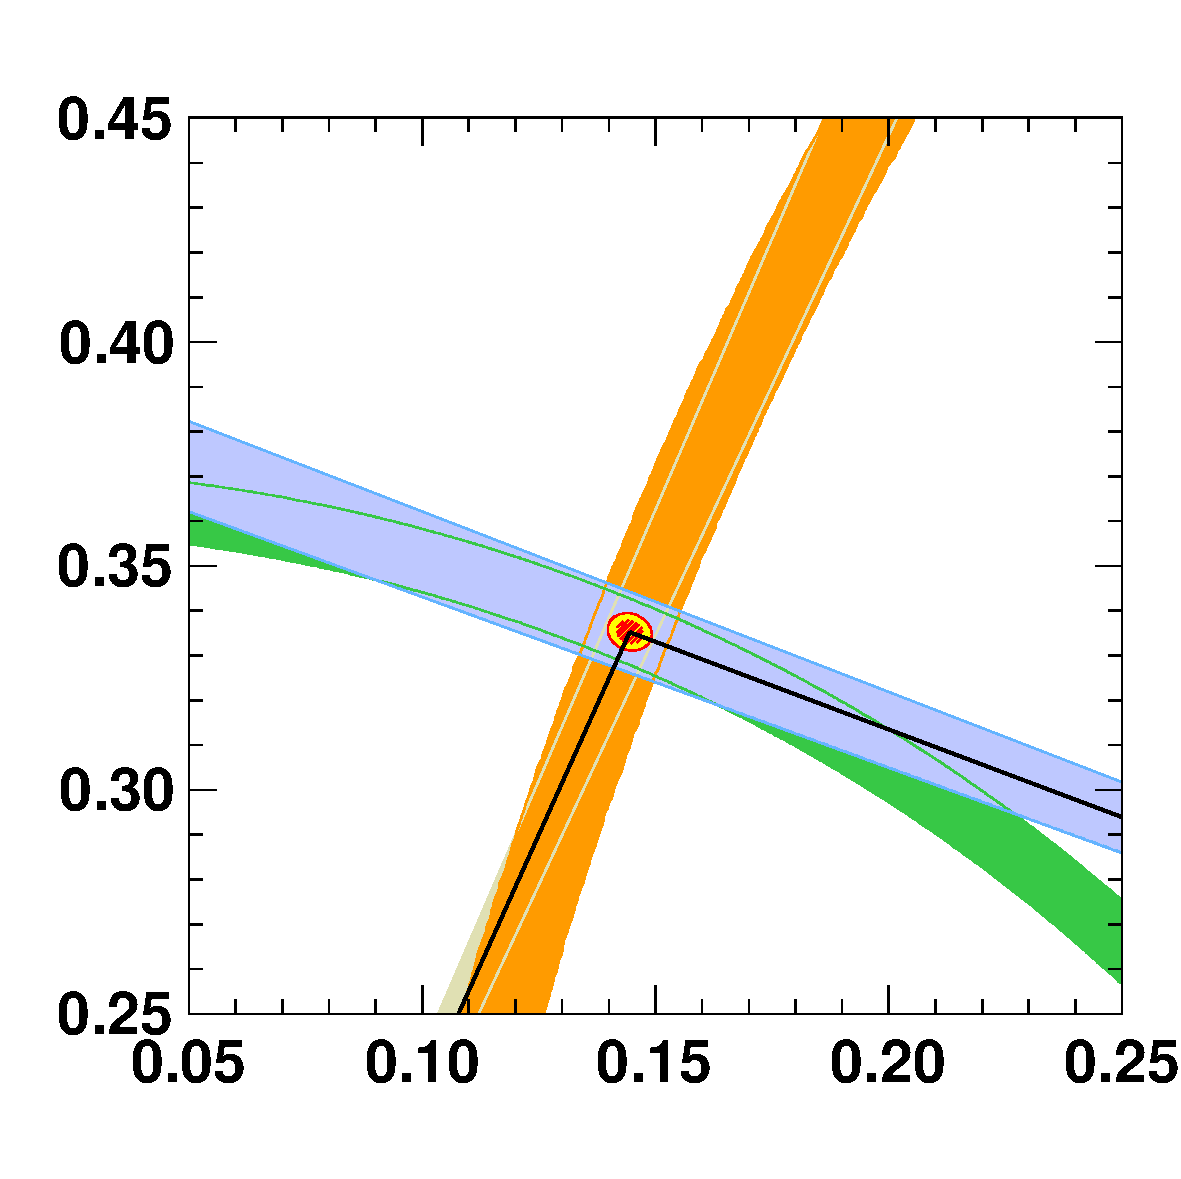
\includegraphics[width=0.26\textwidth]{section1/figs/rhoeta_small_zoom_LHCb_Stage2.pdf}}
\vspace{2.25cm}
\end{minipage}

\caption{\small  Evolving constraints in the $\bar{\rho}-\bar{\eta}$ plane from LHCb measurements and lattice QCD calculations, alone, with current inputs (2018), and the anticipated improvements from the data accumulated by 2025  (23\,fb$^{-1}$) and 2035 (300\,fb$^{-1}$). More information on the fits may be found in Section~\ref{sec:metro-CKM} and~\cite{Bediaga:2018lhg}.
 }
\label{fig:UTprojection}
\end{center}
\end{figure} 
%
\begin{table}[htb]
\caption{\small
Uncertainty on Wilson coefficients and 90\% exclusion limits on New Physics scales for different data samples.  The  $C_9$ analysis is based on the ratio of branching fractions $R_K$ and $R_{K^\ast}$ in the range $1<q^2<6\,{\rm GeV}^2/c^4$.  The $C^\prime_{10}$  analysis exploits the angular observables $S_i$ from the decay $B^0 \to K^{\ast 0} \mu^+\mu^-$ in the ranges $1 < q^2 < 6\,{\rm GeV}^2/c^4$ and  $15 < q^2 < 19\,{\rm GeV}^2/c^4$.   The limits on the scale of New Physics, $\Lambda_{\rm NP}$, are given for the following scenarios: tree-level generic, tree-level minimum flavour violation, loop-level generic and loop-level minimum flavour violation.  More information on the fits may be found in~\cite{Bediaga:2018lhg}.} \label{tab:wilson_sum}
  \begin{center}
  \begin{tabular}{lrrr}\hline\hline
    Integrated Luminosity & $3\invfb$ & $23\invfb$ & $300\invfb$\\ \hline
    \multicolumn{4}{c}{$R_K$ and $R_{K^*}$ measurements}\\\hline
 %   $\sigma^\textrm{stat}(R_K)/R_K~[\%]$ & 12.1 & 3.4 & 0.9\\
 %   $\sigma^\textrm{stat}(R_{K^*})/R_{K^*}~[\%]$ & 15.9 & 4.4 & 1.2\\
    $\sigma(C_9)$ & 0.44 & 0.12 & 0.03\\
    $\Lambda_\textrm{NP}^\textrm{tree\,generic}~[\tev]$ & 40 & 80 & 155\\
    $\Lambda_\textrm{NP}^\textrm{tree\,MFV}~[\tev]$ & 8 & 16 & 31\\
    %$\Lambda_\textrm{NP}^\textrm{loop\,generic}~[\tev]$ & 3.3 & 6.3 & 12.3\\
    $\Lambda_\textrm{NP}^\textrm{loop\,generic}~[\tev]$ & 3 & 6 & 12\\
    $\Lambda_\textrm{NP}^\textrm{loop\,MFV}~[\tev]$ & 0.7 & 1.3 & 2.5\\ \hline
    \multicolumn{4}{c}{$\decay{\Bd}{\Kstarz\mumu}$ angular analysis}\\\hline   
    $\sigma^\textrm{stat}(S_i)$ & 0.034--0.058 & 0.009--0.016 & 0.003--0.004\\
    $\sigma(C_{10}^\prime)$ & 0.31 & 0.15 & 0.06 \\
    $\Lambda_\textrm{NP}^\textrm{tree\,generic}~[\tev]$ & 50 & 75 & 115\\
    $\Lambda_\textrm{NP}^\textrm{tree\,MFV}~[\tev]$ & 10 & 15 & 23\\
    %$\Lambda_\textrm{NP}^\textrm{loop\,generic}~[\tev]$ & 4.0 & 5.8 & 9.2\\
    $\Lambda_\textrm{NP}^\textrm{loop\,generic}~[\tev]$ & 4 & 6 & 9\\
    $\Lambda_\textrm{NP}^\textrm{loop\,MFV}~[\tev]$ & 0.8 & 1.2 & 1.9\\
    \hline\hline
    \end{tabular}
    \end{center}
\end{table}
%
\end{document}